% संपूर्ण मराठी ग्रंथातील प्रकरण 21: अंतर्वेशन प्रमेय
% हा संपादनयोग्य स्रोतखंड आहे. संकलनासाठी संपूर्ण स्रोतसंग्रहातील
% अक्षररूपे, पूर्वभाग, चिन्हव्याख्या आणि आकृती-स्रोत आवश्यक आहेत.
% मूळ: Open Logic Project; मजकूर आणि रूपांतर CC BY 4.0.
% यंत्रानुवाद, दुरुस्ती आणि तपासणी: OpenAI Codex —
% GPT-5.6 Sol आणि GPT-6 Sol, दोन्ही Ultra effort.
% दुरुस्ती-पुनरावलोकन: GPT-6.1 Sol, Ultra effort.
\chapter{अंतर्वेशन प्रमेय}\label{mod:int::chap}









\section{परिचय}\label{mod:int:int:sec}

अंतर्वेशन प्रमेय म्हणजे पुढील निष्कर्ष: समजा
$\Entails \varphi \lif \psi$. मग असे वाक्य~$\chi$ असते की
$\Entails \varphi \lif \chi$ आणि $\Entails \chi \lif \psi$. शिवाय,
$\chi$ मधील प्रत्येक स्थिरांक, फलन आणि विधेय
($\eq$ खेरीज) हे $\varphi$ आणि~$\psi$ या दोन्हींमध्ये आढळते. वाक्य~$\chi$
ला $\varphi$ आणि~$\psi$ यांचे \emph{अंतर्वेशक} म्हणतात.

अंतर्वेशन प्रमेय स्वतःही रंजक आहे; पण त्याचे मुख्य महत्त्व असे की,
उपपत्तीतील परिभाष्यतेविषयीचे निष्कर्ष आणि दोन सुसंगत उपपत्ती एकत्र केल्यावर
मिळणारी उपपत्ती कोणत्या अटींवर सुसंगत असते याविषयीचे निष्कर्ष सिद्ध करण्यासाठी
ते वापरता येते. पहिला निष्कर्ष बेथचे परिभाष्यता प्रमेय म्हणून, तर
दुसरा रॉबिन्सनचे संयुक्त सुसंगतता प्रमेय म्हणून ओळखला जातो.












\section{वाक्याचे विलगीकरण}\label{mod:int:sep:sec}

अंतर्वेशन प्रमेयाची सिद्धता सुरू करण्यापूर्वी थोडी पूर्वतयारी आवश्यक आहे.
$\varphi$ आणि~$\psi$ यांचे अंतर्वेशक म्हणजे असे वाक्य~$\chi$ की
$\varphi \Entails \chi$ आणि $\chi \Entails \psi$. प्रतिपरिवर्तनानुसार, यांपैकी
नंतरचे विधान तेव्हा आणि केवळ तेव्हाच खरे असते, जेव्हा $\lnot \psi
\Entails \lnot \chi$. हा गुणधर्म असलेले वाक्य~$\chi$ हे $\varphi$
आणि~$\lnot \psi$ यांना \emph{विलग करते} असे म्हणतात. म्हणून $\varphi$ आणि~$\psi$
यांचे अंतर्वेशक शोधणे म्हणजे $\varphi$ आणि~$\lnot \psi$ यांना विलग करणारे
वाक्य शोधणेच होय. नेहमीप्रमाणे, याचे व्यापक रूप विचारात घेणे उपयोगी
ठरेल: वाक्यांच्या दोन \emph{संचांना} विलग करणारे वाक्य.

\begin{defn}
वाक्य~$\chi$ हे वाक्यसंच~$\Gamma$ आणि~$\Delta$ यांना \emph{विलग करते}
तेव्हा आणि केवळ तेव्हाच, जेव्हा $\Gamma \Entails \chi$ आणि $\Delta
\Entails \lnot \chi$. असे कोणतेही वाक्य अस्तित्वात नसेल, तर
$\Gamma$ आणि~$\Delta$ यांना \emph{अविलगनीय} म्हणतात.
\end{defn}

$\Gamma$, $\Delta$ आणि~$\chi$ यांच्या प्रतिमान-वर्गांमधील समावेशन-संबंध
खाली दर्शवले आहेत:
\begin{figure}[h]
  \centering
  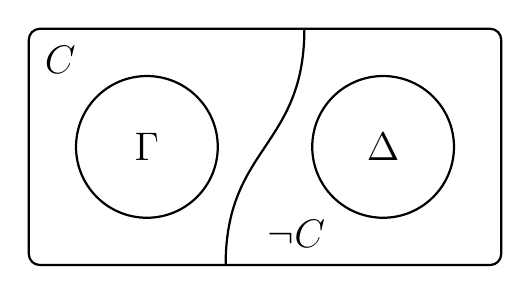
\begin{tikzpicture}[node distance=2cm, auto, thick]
    \draw [rounded corners] (0,0) -- (6,0) -- (6,3) -- (0,3) --  cycle;
    \draw (1.5,1.5) circle (0.9cm);
    \draw (4.5,1.5) circle (0.9cm);
    \path node at (1.5,1.5) {\Large $\Gamma$};
    \path node at (4.5,1.5) {\Large $\Delta$};
    \path node at (0.4,2.6) {\Large $\formula{C}$};
    \path node at (3.4,0.4) {\Large $\lnot \formula{C}$};
    \draw (2.5,0) .. controls (2.5,1.5) and (3.5,1.5) .. (3.5,3);
  \end{tikzpicture}
  \caption{$\chi$ हे $\Gamma$ आणि $\Delta$ यांना विलग करते}
  \label{mod:int:sep:fig:sep}
\end{figure}


\begin{lem}\label{mod:int:sep:lem:sep1}
समजा $\Lang{L}_0$ या भाषेत $\Gamma$ आणि~$\Delta$ या \emph{दोन्हींमध्ये}
आढळणारे प्रत्येक स्थिरांक, फलन आणि विधेय ($\doteq$
खेरीज) येते; आणि प्रत्येक $n \ge 0$ साठी अनंत नवीन स्थिरांक
$\Obj c_n$ जोडून $\Lang{L}'_0$ मिळवली आहे. मग $\Gamma$ आणि~$\Delta$ हे
$\Lang{L}_0$ मध्ये अविलगनीय असतील, तर ते $\Lang{L}'_0$ मध्येही अविलगनीय
असतात.
\end{lem}

\begin{proof}
विरोधाभास पद्धतीने सिद्ध करू: विरुद्धार्थी असे समजा की $\Gamma$ आणि
$\Delta$ हे $\Lang{L}'_0$ मध्ये विलगनीय आहेत. मग एखाद्या $\chi \in
\Lang{L}_0$ साठी $\Gamma \Entails \Subst{\chi}{c}{x}$ आणि $\Delta
\Entails \lnot \Subst{\chi}{c}{x}$ असते (येथे $c$ हे नवीन स्थिरांक
आहे---$\chi$ मध्ये अशी एकाहून अधिक नवीन स्थिरांक असलेले प्रकरणही यासारखेच
आहे). संहततेनुसार, $\Gamma$ चा \emph{सांत} उपसंच~$\Gamma_0$ आणि
$\Delta$ चा सांत उपसंच~$\Delta_0$ असे आहेत की $\Gamma_0 \Entails
\Subst{\chi}{c}{x}$ आणि $\Delta_0 \Entails \lnot \Subst{\chi}{c}{x}$.
$\Gamma_0$ मधील सर्व सूत्रांचा संयोग~$\varphi_{G}$ आणि $\Delta_0$ मधील सर्व
सूत्रांचा संयोग~$\varphi_{H}$ असू द्या. मग
\begin{align*}
  \varphi_{G} & \Entails \Subst{\chi}{c}{x}, & \varphi_{H}  \Entails \lnot \Subst{\chi}{c}{x}.
\end{align*}
पहिल्या विधानावर सामान्यीकरण लावल्यास $\varphi_{G} \Entails \lforall[x][\chi]$
मिळते; आणि दुसऱ्यावर प्रतिपरिवर्तन लावल्यास $\Subst{\chi}{c}{x}
\Entails \lnot \varphi_{H}$ मिळते, म्हणून $\lforall[x][\chi] \Entails \lnot \varphi_{H}$.

पुन्हा प्रतिपरिवर्तन केल्यास $\varphi_{H} \Entails \lnot \lforall[x][\chi]$
मिळते. एकस्वनिकतेनुसार,
\begin{align*}
  \Gamma &\Entails \lforall[x][\chi], &
  \Delta & \Entails \lnot \lforall[x][\chi],
\end{align*}
त्यामुळे $\lforall[x][\chi]$ हे $\Lang{L}_0$ मध्ये $\Gamma$ आणि~$\Delta$
यांना विलग करते.
\end{proof}

\begin{lem}\label{mod:int:sep:lem:sep2}
समजा $\Gamma \cup \{ \lexists[x][\varphi_{S}] \}$ आणि~$\Delta$ हे अविलगनीय
आहेत, आणि $c$ हे $\Gamma$, $\Delta$ किंवा~$\varphi_{S}$ यांपैकी कशातही नसलेले नवीन
स्थिरांक आहे. मग $\Gamma \cup \{ \lexists[x][\varphi_{S}],
\Subst{\varphi_{S}}{c}{x} \}$ आणि~$\Delta$ हेही अविलगनीय असतात.
\end{lem}

\begin{proof}
विरोधाभासासाठी असे समजा की $\chi$ हे $\Gamma \cup \{ \lexists[x][\varphi_{S}],
\Subst{\varphi_{S}}{c}{x}\}$ आणि~$\Delta$ यांना विलग करते, पण त्याच वेळी
$\Gamma \cup \{\lexists[x]{\varphi_{S}} \}$ आणि~$\Delta$ हे अविलगनीय आहेत. दोन
प्रकरणे वेगळी करू:
\begin{enumerate}
\item $\chi$ मध्ये $c$ आढळत नाही: या प्रकरणात $\Gamma \cup
  \{\lexists[x][\varphi_{S}], \lnot\chi \}$ हा संच पूर्ततायोग्य असतो (अन्यथा
  $\chi$ हे $\Gamma \cup \{\lexists[x][\varphi_{S}] \}$ आणि~$\Delta$ यांना विलग
  करेल). $\Subst{\varphi_{S}}{c}{x}$ ची भर घातल्यानंतरही तो पूर्ततायोग्य राहतो;
  म्हणून अखेरीस $\chi$ हे $\Gamma \cup \{ \lexists[x][\varphi_{S}],
  \Subst{\varphi_{S}}{c}{x} \}$ आणि~$\Delta$ यांना विलग करत नाही.
\item $\chi$ मध्ये $c$ आढळते, त्यामुळे $\chi$ चे रूप
  $\Subst{\chi}{c}{x}$ असते. मग
  \[  \Gamma \cup \{ \lexists[x][\varphi_{S}], \Subst{\varphi_{S}}{c}{x}\} \Entails \Subst{\chi}{c}{x},
  \]
  असे असते. यावरून निगमन प्रमेय आणि सामान्यीकरण यांच्या साहाय्याने
  $\Gamma, \lexists[x][\varphi_{S}] \Entails \lforall[x][(\varphi_{S} \lif \chi)]$ आणि
  अखेरीस $\Gamma \cup \{ \lexists[x][\varphi_{S}] \} \Entails
  \lexists[x][\chi]$ मिळते. दुसरीकडे, $\Delta \Entails \lnot
  \Subst{\chi}{c}{x}$; म्हणून सामान्यीकरणाने $\Delta \Entails \lnot
  \lexists[x][\chi]$. त्यामुळे $\Gamma \cup \{\lexists[x][\varphi_{S}] \}$
  आणि~$\Delta$ हे विलगनीय ठरतात, आणि हा विरोधाभास आहे.
\end{enumerate}
\end{proof}












\section{क्रेगचे अंतर्वेशन प्रमेय}\label{mod:int:prf:sec}

\begin{thm}[क्रेगचे अंतर्वेशन प्रमेय]
\label{mod:int:prf:thm:interpol}
$\Entails \varphi \lif \psi$ असेल, तर असे वाक्य~$\chi$ असते की
$\Entails \varphi \lif \chi$ आणि $\Entails \chi \lif \psi$; तसेच $\chi$ मधील
प्रत्येक स्थिरांक, फलन आणि विधेय ($\eq$ खेरीज) हे
$\varphi$ आणि~$\psi$ या दोन्हींमध्ये आढळते. वाक्य~$\chi$ ला $\varphi$ आणि~$\psi$
यांचे \emph{अंतर्वेशक} म्हणतात.
\end{thm}

\begin{proof}
समजा $\Lang{L}_1$ ही $\varphi$ ची भाषा आणि $\Lang{L}_2$ ही $\psi$ ची भाषा
आहे. $\Lang{L}_0 = \Lang{L}_1 \cap \Lang{L}_2$ असे ठेवू. प्रत्येक
$i \in \{0, 1, 2 \}$ साठी, $\Lang{L}_i$ मध्ये अनंत नवीन स्थिरांक
$\Obj c_0, \Obj c_1, \Obj c_2, \dots$ जोडून $\Lang{L}'_i$ मिळवू.

$\varphi$ अपूर्ततायोग्य असेल, तर $\lexists[x][\eq/[x][x]]$ हे अंतर्वेशक आहे.
$\lnot \psi$ अपूर्ततायोग्य असेल (आणि म्हणून $\psi$ वैध असेल), तर
$\lexists[x][\eq[x][x]]$ हे अंतर्वेशक आहे. म्हणून $\varphi$ आणि~$\lnot \psi$
ही दोन्ही पूर्ततायोग्य आहेत असेही आपण मानू शकतो.

अंतर्वेशन प्रमेयाचे प्रतिपरिवर्तित विधान सिद्ध करण्यासाठी, $\varphi$ आणि~$\psi$
यांचे कोणतेही अंतर्वेशक नाही असे गृहीत धरू. दुसऱ्या शब्दांत, $\{\varphi\}$
आणि~$\{\lnot \psi\}$ हे $\Lang{L}_0$ मध्ये अविलगनीय आहेत असे गृहीत धरू.

$(\{ \varphi \}, \{\lnot\psi\})$ या जोडीचा विस्तार करून महत्तम अविलगनीय जोडी
$(\Gamma^*, \Delta^*)$ मिळवणे हे आपले उद्दिष्ट आहे. $\varphi_0$, $\varphi_1$,
$\varphi_2$, \dots{} हे $\Lang{L}_1$ च्या वाक्यांचे प्रगणन आणि $\psi_0$,
$\psi_1$, $\psi_2$, \dots{} हे $\Lang{L}_2$ च्या वाक्यांचे प्रगणन असू
द्या. प्रत्येक $n \ge 0$ साठी वाक्यांच्या संचांचे दोन वर्धमान अनुक्रम
$(\Gamma_n, \Delta_n)$ पुढीलप्रमाणे परिभाषित करू. $\Gamma_0 = \{ \varphi\}$
आणि $\Delta_0 = \{\lnot \psi \}$ असे ठेवू. $(\Gamma_n, \Delta_n)$ आधीच
परिभाषित आहेत असे मानून $\Gamma_{n+1}$ आणि $\Delta_{n+1}$ पुढीलप्रमाणे
परिभाषित करू:
\begin{enumerate}
\item $\Gamma_n \cup \{\varphi_n \}$ आणि~$\Delta_n$ हे $\Lang{L}'_0$ मध्ये
  अविलगनीय असतील, तर $\varphi_n$ चा $\Gamma_{n+1}$ मध्ये समावेश करा. शिवाय,
  $\varphi_n$ हे $\lexists[x][\varphi_{S}]$ या रूपातील अस्तित्ववाची सूत्र असेल,
  तर $\Gamma_n$, $\Delta_n$, $\varphi_n$ किंवा~$\psi_n$ यांपैकी कशातही न आढळणारे
  नवीन स्थिरांक~$c$ निवडा आणि $\Subst{\varphi_{S}}{c}{x}$ चा $\Gamma_{n+1}$
  मध्ये समावेश करा.
\item $\Gamma_{n+1}$ आणि~$\Delta_n \cup \{\psi_n \}$ हे $\Lang{L}'_0$
  मध्ये अविलगनीय असतील, तर $\psi_n$ चा $\Delta_{n+1}$ मध्ये समावेश करा.
  शिवाय, $\psi_n$ हे $\lexists[x][\varphi_{S}]$ या रूपातील अस्तित्ववाची सूत्र
  असेल, तर $\Gamma_{n+1}$, $\Delta_n$, $\varphi_n$ किंवा~$\psi_n$ यांपैकी कशातही
  न आढळणारे नवीन स्थिरांक~$c$ निवडा आणि $\Subst{\varphi_{S}}{c}{x}$ चा
  $\Delta_{n+1}$ मध्ये समावेश करा.
\end{enumerate}
शेवटी, पुढील व्याख्या करू:
\begin{align*}
  \Gamma^* & = \bigcup_{n\ge 0} \Gamma_n, &
  \Delta^* & = \bigcup_{n\ge 0} \Delta_n.
\end{align*}
आता $n$ वरील युगपत् विगमनाने पुढील गोष्टी सिद्ध करता येतात:
\begin{enumerate}
\item\label{mod:int:prf:part-a} $\Gamma_n$ आणि~$\Delta_n$ हे $\Lang{L}'_0$ मध्ये
  अविलगनीय आहेत;
\item\label{mod:int:prf:part-b} $\Gamma_{n+1}$ आणि~$\Delta_n$ हे $\Lang{L}'_0$
  मध्ये अविलगनीय आहेत.
\end{enumerate}
\ref{mod:int:prf:part-a} चा आधार \ref{mod:int:sep:lem:sep1} मुळे मिळतो. \ref{mod:int:prf:part-b}
साठी तीन प्रकरणे वेगळी करावी लागतात:
\begin{enumerate}
\item $\Gamma_0 \cup \{\varphi_0 \}$ आणि~$\Delta_0$ हे विलगनीय असतील, तर
  $\Gamma_1 = \Gamma_0$; त्यामुळे \ref{mod:int:prf:part-b} म्हणजे फक्त
  \ref{mod:int:prf:part-a} होय.
\item $\Gamma_1 = \Gamma_0 \cup\{ \varphi_0\}$ असेल, तर रचनेनुसार
  $\Gamma_1$ आणि~$\Delta_0$ हे अविलगनीय आहेत.
\item आता फक्त $\varphi_0$ अस्तित्ववाची असलेले प्रकरण उरते; तेव्हा
  $\Gamma_1 = \Gamma_0 \cup \{ \lexists[x][\varphi_{S}], \Subst{\varphi_{S}}{c}{x}
  \}$. रचनेनुसार $\Gamma_0 \cup \{ \lexists[x][\varphi_{S}]\}$ आणि~$\Delta_0$
  हे अविलगनीय आहेत; म्हणून \ref{mod:int:sep:lem:sep2} नुसार $\Gamma_0 \cup
  \{ \lexists[x][\varphi_{S}], \Subst{\varphi_{S}}{c}{x} \}$ आणि~$\Delta_0$ हेही
  अविलगनीय आहेत.
\end{enumerate}
यावरून वरील \ref{mod:int:prf:part-a} आणि \ref{mod:int:prf:part-b} यांच्यासाठी विगमनाचा आधार
पूर्ण होतो. आता विगमन-पायरी पाहू. \ref{mod:int:prf:part-a} साठी, $\Delta_{n+1} =
\Delta_n \cup \{ \psi_n \}$ असेल, तर रचनेनुसार $\Gamma_{n+1}$ आणि
$\Delta_{n+1}$ हे अविलगनीय आहेत ($\psi_n$ अस्तित्ववाची असतानाही
\ref{mod:int:sep:lem:sep2} नुसार हेच मिळते); आणि $\Delta_{n+1} = \Delta_n$
असेल ($\Gamma_{n+1}$ आणि~$\Delta_n \cup \{\psi_n\}$ विलगनीय असल्यामुळे),
तर \ref{mod:int:prf:part-b} साठीचे विगमन-गृहीतक वापरतो. \ref{mod:int:prf:part-b} च्या
विगमन-पायरीसाठी, $\Gamma_{n+2} = \Gamma_{n+1} \cup \{\varphi_{n+1} \}$
असेल, तर रचनेनुसार $\Gamma_{n+2}$ आणि~$\Delta_{n+1}$ हे अविलगनीय आहेत
($\varphi_{n+1}$ अस्तित्ववाची असतानाही \ref{mod:int:sep:lem:sep2} नुसार हेच
मिळते); आणि $\Gamma_{n+2} = \Gamma_{n+1}$ असेल, तर नुकतेच सिद्ध केलेले
\ref{mod:int:prf:part-a} चे विगमन-प्रकरण वापरतो. अशा रीतीने \ref{mod:int:prf:part-a} आणि
\ref{mod:int:prf:part-b} यांवरील विगमन पूर्ण होते.

यावरून $\Gamma^*$ आणि~$\Delta^*$ हे अविलगनीय आहेत. तसे नसते, तर
संहततेनुसार असा $n \ge 0$ असता की $\Gamma_n$ आणि~$\Delta_n$ विलगनीय
असते, आणि हे \ref{mod:int:prf:part-a} च्या विरुद्ध आहे. विशेषतः, $\Gamma^*$ आणि
$\Delta^*$ हे सुसंगत आहेत: कारण यांपैकी अनुक्रमे पहिला किंवा दुसरा विसंगत
असता, तर $\lexists[x][\eq/[x][x]]$ किंवा
$\lforall[x][\eq[x][x]]$ यांनी ते विलग झाले असते.

आता $\Gamma^*$ हा $\Lang{L}'_1$ मध्ये महत्तम सुसंगत आहे आणि त्याचप्रमाणे
$\Delta^*$ हा $\Lang{L}'_2$ मध्ये महत्तम सुसंगत आहे, हे दाखवू. पहिल्यासाठी,
एखाद्या $n \ge 0$ करिता $\varphi_n \notin \Gamma^*$ आणि $\lnot \varphi_n
\notin \Gamma^*$ असे समजा. $\varphi_n \notin \Gamma^*$ असल्यास $\Gamma_n
\cup \{\varphi_n \}$ हा $\Delta_n$ पासून विलगनीय असतो; म्हणून असे
$\chi \in \Lang{L}'_0$ असते की पुढील दोन्ही विधाने खरी असतात:
\begin{align*}
  \Gamma^* & \Entails \varphi_n \lif \chi, &
  \Delta^* & \Entails \lnot \chi.
\end{align*}
त्याचप्रमाणे, $\lnot \varphi_n \notin \Gamma^*$ असेल, तर असे $\chi' \in
\Lang{L}'_0$ असते की पुढील दोन्ही विधाने खरी असतात:
\begin{align*}
  \Gamma^* & \Entails \lnot \varphi_n \lif \chi', &
  \Delta^* & \Entails \lnot \chi'.
\end{align*}
विधान तर्कशास्त्रानुसार $\Gamma^* \Entails \chi \lor \chi'$ आणि
$\Delta^* \Entails \lnot (\chi \lor \chi')$; म्हणून $\chi \lor \chi'$ हे
$\Gamma^*$ आणि~$\Delta^*$ यांना विलग करते. यासारख्याच युक्तिवादाने
$\Delta^*$ हा महत्तम असल्याचे सिद्ध होते.

शेवटी, $\Gamma^* \cap \Delta^*$ हा $\Lang{L}'_0$ मध्ये महत्तम सुसंगत
आहे हे दाखवू. तो सुसंगत संचांचा छेद असल्यामुळे उघडपणे सुसंगत आहे. महत्तमता
दाखवण्यासाठी $\varphi_{S} \in \Lang{L}'_0$ असू द्या. आता $\Gamma^*$ हा
$\Lang{L'_1} \supseteq \Lang{L'_0}$ मध्ये महत्तम आहे आणि त्याचप्रमाणे
$\Delta^*$ हा $\Lang{L'_2} \supseteq \Lang{L'_0}$ मध्ये महत्तम आहे.
त्यामुळे $\varphi_{S} \in \Gamma^*$ किंवा $\lnot \varphi_{S} \in \Gamma^*$, आणि
$\varphi_{S} \in \Delta^*$ किंवा $\lnot \varphi_{S} \in \Delta^*$. जर $\varphi_{S} \in
\Gamma^*$ आणि $\lnot \varphi_{S} \in \Delta^*$ असते, तर $\varphi_{S}$ ने $\Gamma^*$
आणि~$\Delta^*$ यांना विलग केले असते; आणि जर $\lnot \varphi_{S} \in \Gamma^*$
आणि $\varphi_{S} \in \Delta^*$ असते, तर $\lnot \varphi_{S}$ ने $\Gamma^*$ आणि~$\Delta^*$
यांना विलग केले असते. म्हणून एकतर $\varphi_{S} \in \Gamma^* \cap \Delta^*$
किंवा $\lnot \varphi_{S} \in \Gamma^* \cap \Delta^*$; त्यामुळे $\Gamma^* \cap
\Delta^*$ हा महत्तम आहे.

$\Gamma^*$ हा महत्तम सुसंगत असल्यामुळे त्याला असे प्रतिमान
$\Struct{M}'_1$ असते की त्याचा प्रांत~$\Domain{M'_1}$ हा
स्थिरांकाची अर्थनिर्धारणे असलेल्या सर्व आणि केवळ $\Assign{c}{M'_1}$
या घटकांचा बनलेला असतो---अगदी संपूर्णता प्रमेयाच्या सिद्धतेप्रमाणे
(\ref{fol:com:cth:thm:completeness}). त्याचप्रमाणे, $\Delta^*$ ला
असे प्रतिमान~$\Struct{M}'_2$ असते की त्याचा प्रांत~$\Domain{M'_2}$
हा स्थिरांकाची $\Assign{c}{M'_2}$ ही अर्थनिर्धारणे घेऊन बनलेला असतो.

$\Lang{L'_1} \setminus \Lang{L'_0}$ मधील स्थिरांक, फलने
आणि विधेये यांची अर्थनिर्धारणे वगळून $\Struct{M'_1}$ पासून
$\Struct{M_1}$ मिळवू; आणि त्याचप्रमाणे $\Struct{M_2}$ मिळवू. मग
$h(\Assign{c}{M'_1}) = \Assign{c}{M'_2}$ अशी व्याख्या असलेले प्रतिचित्रण
$h \colon M_1 \to M_2$ हे $\Lang{L}'_0$ मधील समरूपण आहे, कारण दाखवल्याप्रमाणे
$\Gamma^* \cap \Delta^*$ हा $\Lang{L}'_0$ मध्ये महत्तम सुसंगत आहे. हे
पुढील कारणाने मिळते: कोणतेही $\Lang{L}'_0$-वाक्य हे एकतर $\Gamma^*$
आणि~$\Delta^*$ या दोन्हींचा घटक असते, किंवा दोन्हींपैकी कशाचाही नसते;
म्हणून $\Assign{c}{M'_1} \in \Assign{P}{M'_1}$ तेव्हा आणि केवळ तेव्हाच,
जेव्हा $\Atom{P}{c} \in \Gamma^*$, तेव्हा आणि केवळ तेव्हाच, जेव्हा
$\Atom{P}{c} \in \Delta^*$, तेव्हा आणि केवळ तेव्हाच, जेव्हा
$\Assign{c}{M'_2} \in \Assign{P}{M'_2}$. समरूपणांनी पूर्ण केलेल्या इतर
अटीही याच रीतीने सिद्ध करता येतात.

आता भाषा~$\Lang{L_1} \cup \Lang{L_2}$ साठी प्रतिमान~$\Struct{M}$
पुढीलप्रमाणे परिभाषित करू:
\begin{enumerate}
\item प्रांत~$\Domain{M}$ म्हणजे $\Domain{M_2}$, म्हणजेच सर्व
  $\Assign{c}{M'_2}$ घटकांचा संच;
\item विधेय~$P$ हे $\Lang{L_2} \setminus \Lang{L_1}$ मध्ये
  असेल, तर $\Assign{P}{M} = \Assign{P}{M'_2}$;
\item विधेय~$P$ हे $\Lang{L}_1\setminus \Lang{L}_2$ मध्ये असेल, तर
  $\Assign{P}{M} = h(\Assign{P}{M'_1})$, म्हणजे
  $\tuple{\Assign{c_1}{M'_2}, \dots, \Assign{c_n}{M'_2}} \in
  \Assign{P}{M}$ तेव्हा आणि केवळ तेव्हाच, जेव्हा
  $\tuple{\Assign{c_1}{M'_1}, \dots, \Assign{c_n}{M'_1}} \in
  \Assign{P}{M'_1}$.

\item विधेय~$P$ हे $\Lang{L}_0$ मध्ये असेल, तर $\Assign{P}{M} =
  \Assign{P}{M'_2} = h(\Assign{P}{M'_1})$.
\item $\Lang{L}_1 \cup \Lang{L}_2$ ची फलने, त्यांत
  स्थिरांक धरून, याच रीतीने हाताळली जातात.
\end{enumerate}

शेवटी, सूत्रे वरील विगमनाने असे दाखवता येते की $\Struct{M}$ हे
$\Lang{L'_1}$ च्या सर्व सूत्रे बाबत $\Struct{M'_1}$ शी आणि
$\Lang{L'_2}$ च्या सर्व सूत्रे बाबत $\Struct{M'_2}$ शी सहमत असते.
विशेषतः, $\Struct{M} \Entails \Gamma^* \cup \Delta^*$; त्यामुळे
$\Struct{M} \Entails \varphi$ आणि $\Struct{M} \Entails \lnot\psi$, तसेच
$\not\Entails \varphi \lif \psi$. याने क्रेगच्या अंतर्वेशन प्रमेयाची सिद्धता
पूर्ण होते.
\end{proof}












\section{परिभाष्यता प्रमेय}\label{mod:int:def:sec}

अंतर्वेशन प्रमेयाचा एक महत्त्वाचा उपयोग म्हणजे बेथचे परिभाष्यता प्रमेय.
$n$-स्थानी संबंध~$R$ परिभाषित करण्यासाठी आपण $R$ चा समावेश नसलेले आणि
$n$ मुक्त चले असलेले सूत्र~$\chi$ देऊ शकतो. ही $\chi$ च्या
साहाय्याने केलेली $R$ ची \emph{स्पष्ट} परिभाषा असेल. मग असेही म्हणता येते
की $n$-स्थानी विधेय~$P$ असलेल्या भाषा मधील
उपपत्ती~$\Sigma(P)$ मध्ये औपचारिक स्पष्ट परिभाषा समाविष्ट असेल (किंवा निदान
ती परिभाषा त्या उपपत्तीतून निष्पन्न होत असेल), म्हणजे
\[\Sigma(P) \Entails \lforall[x_1][\dots
  \lforall[x_n][(\Atom{P}{x_1,\dots, x_n} \liff \chi(x_1, \dots,
    x_n))]].
\]
तर ती उपपत्ती $P$ ला स्पष्टपणे परिभाषित करते. परंतु एखादा संबंध
परिभाषित करण्याच्या---म्हणजे तो पूर्णपणे निर्धारित करण्याच्या---मार्गांपैकी
स्पष्ट परिभाषा हा केवळ एक मार्ग आहे. कोणत्याही प्रतिमानात भाषा च्या उर्वरित भागाचा अर्थबोध
दिला की $P$ चा अर्थबोध निश्चित होईल, अशीही एखादी उपपत्ती असू शकते.
परिभाष्यता प्रमेय असे सांगते की उपपत्ती जेव्हा या रीतीने $P$ चा अर्थबोध
निश्चित करते---जेव्हा ती $P$ ला \emph{अंतर्निहितपणे परिभाषित करते}---तेव्हा
ती त्याला स्पष्टपणेही परिभाषित करते.

\begin{defn}
समजा, विधेय~$P$ चा समावेश नसलेली $\Lang{L}$ ही भाषा आहे. $\Lang{L}
\cup \{P\}$ मधील वाक्यांचा संच $\Sigma(P)$ हा $P$ ला
\emph{स्पष्टपणे परिभाषित करतो}, जर आणि केवळ जर $\Lang{L}$ मधील असे
सूत्र~$\chi(x_1, \dots, x_n)$ असेल की
\[\Sigma(P) \Entails \lforall[x_1][\dots
  \lforall[x_n][(\Atom{P}{x_1,\dots, x_n} \liff \chi(x_1, \dots,
    x_n))]].
\]
\end{defn}

\begin{defn}
समजा, विधेये~$P$ आणि~$P'$ यांचा समावेश नसलेली
$\Lang{L}$ ही भाषा आहे. $\Lang{L} \cup \{P\}$ मधील
वाक्यांचा संच $\Sigma(P)$ हा $P$ ला \emph{अंतर्निहितपणे परिभाषित
करतो}, जर आणि केवळ जर
\[\Sigma(P) \cup \Sigma(P') \Entails \lforall[x_1][\dots
  \lforall[x_n][(\Atom{P}{x_1,\dots, x_n} \liff \Atom{P'}{x_1,\dots,
      x_n})]],
\]
जेथे $\Sigma(P')$ हा $\Sigma(P)$ मध्ये सर्वत्र $P$ च्या जागी $P'$ घालून
मिळणारा संच आहे.
\end{defn}

दुसऱ्या शब्दांत, कोणतेही प्रतिमान $\Struct{M}$ आणि $R, R' \subseteq
\Domain{M}^n$ यांच्यासाठी, $\Expan{M}{R} \Entails \Sigma(P)$ आणि
$\Expan{M}{R'} \Entails \Sigma(P')$ हे दोन्ही खरे असतील, तर $R=R'$;
येथे $\Expan{M}{R}$ ही $\Lang{L}$ च्या $\Lang{L} \cup \{P\}$ या
विस्तारासाठीची अशी संरचना~$\Struct{M'}$ आहे की
$\Assign{P}{M'} = R$, आणि $\Expan{M}{R'}$ साठीही तसेच.

\begin{thm}[बेथचे परिभाष्यता प्रमेय] $\Lang{L}
  \cup\{P\}$-सूत्रांचा संच $\Sigma(P)$ हा $P$ ला अंतर्निहितपणे
  परिभाषित करतो, जर आणि केवळ जर $\Sigma(P)$ हा $P$ ला स्पष्टपणे परिभाषित करतो.

\end{thm}

\begin{proof}
$\Sigma(P)$ हा $P$ ला स्पष्टपणे परिभाषित करत असेल, तर पुढील दोन्ही निष्पन्न होतात:
\begin{align*}
  \Sigma(P) & \Entails & \lforall[x_1][\dots \lforall[x_n]
    [(\Atom{P}{x_1,\dots, x_n} \liff \chi(x_1,\dots,x_n))]]\\
  \Sigma(P') & \Entails & \lforall[x_1][\dots \lforall[x_n]
    [(\Atom{P'}{x_1,\dots, x_n} \liff \chi(x_1,\dots,x_n))]]
\end{align*}
आणि निष्कर्ष मिळतो. उलट दिशेसाठी, समजा $\Sigma(P)$ हा $P$ ला
अंतर्निहितपणे परिभाषित करतो. प्रथम आपण $\Lang{L}$ मध्ये स्थिरांक
$c_1$, \dots,~$c_n$ समाविष्ट करतो. मग
\[\Sigma(P) \cup \Sigma(P') \Entails
\Atom{P}{c_1, \dots, c_n} \to  \Atom{P'}{c_1, \dots, c_n}.
\]
संहततेनुसार, असे सांत संच $\Delta_0 \subseteq \Sigma(P)$ आणि
$\Delta_1 \subseteq \Sigma(P')$ असतात की
\[\Delta_0 \cup \Delta_1 \Entails
\Atom{P}{c_1, \dots, c_n} \to \Atom{P'}{c_1, \dots, c_n}.
\]
$\theta(P)$ हा अशा सर्व वाक्ये $\varphi(P)$ चा संयोग समजू की एकतर
$\varphi(P) \in \Delta_0$ किंवा $\varphi(P') \in \Delta_1$; आणि $\theta(P')$ हा अशा
सर्व वाक्ये $\varphi(P')$ चा संयोग समजू की एकतर $\varphi(P) \in \Delta_0$
किंवा $\varphi(P') \in \Delta_1$. मग $\theta(P) \land
\theta(P') \Entails \Atom{P}{c_1, \dots, c_n} \to \Atom{P'}{c_1, \dots, c_n}$.

प्रत्येक विधेय $\Entails$ च्या एका बाजूला येईल अशा रीतीने याची
पुनर्मांडणी करता येते:
\[\theta(P) \land \Atom{P}{c_1, \dots, c_n} \Entails
\theta(P') \to \Atom{P'}{c_1, \dots, c_n}.
\]
क्रेगच्या अंतर्वेशन प्रमेयानुसार $P$ किंवा $P'$ यांचा समावेश नसलेले असे
वाक्य $\chi(c_1,\dots, c_n)$ असते की
\begin{align*}
  \theta(P) \land \Atom{P}{c_1, \dots, c_n} & \Entails \chi(c_1,\dots, c_n); \\
  \chi(c_1,\dots, c_n) & \Entails \theta(P') \to \Atom{P'}{c_1, \dots, c_n}.
\end{align*}
या दोन निष्पन्नतांपैकी पहिलीवरून $\theta(P) \Entails
\Atom{P}{c_1,\dots, c_n} \lif \chi(c_1,\dots, c_n)$ मिळते. आणि दुसरीवरून,
$\Lang{L} \cup \{P\}$-प्रतिमान $\Expan{M}{R} \Entails \varphi(P)$ असेल जर
आणि केवळ जर संबंधित $\Lang{L} \cup \{P'\}$-प्रतिमान
$\Expan{M}{R} \models \varphi(P')$ असेल, त्यामुळे
$\chi(c_1,\dots, c_n) \Entails \theta(P) \lif \Atom{P}{c_1,\dots, c_n}$ मिळते,
आणि त्यावरून
\[\theta(P) \Entails \chi(c_1,\dots,c_n) \to \Atom{P}{c_1,\dots, c_n}.
\]
दोन्ही एकत्र केल्यावर $\theta(P) \Entails \Atom{P}{c_1,\dots, c_n}
\liff \chi(c_1, \dots, c_n)$ मिळते; आणि एकस्वनिकता व सामान्यीकरण यांनुसार पुढीलही मिळते:
\[\Sigma(P) \Entails
\lforall[x_1][\dots\lforall[x_n][(\Atom{P}{x_1,\dots, x_n} \liff
    \chi(x_1,\dots, x_n))]].
\]
\end{proof}



